\documentclass[12pt]{article}
\usepackage{natbib}
\usepackage{hyperref}
\usepackage{graphicx}
\usepackage{subcaption}
\usepackage{amssymb,amsmath,amsthm}
\usepackage{xcolor}
\usepackage{xspace}
\usepackage[nameinlink,capitalize]{cleveref}
\usepackage{cleveref}
\usepackage{geometry}
\usepackage{pdflscape}

\usepackage{xspace}
\newcommand{\Rlogo}{\protect
\includegraphics[height=2ex,keepaspectratio]
{pix/Rlogo.pdf}\xspace}

\newcommand{\comment}{\showcomment}
%% \newcommand{\comment}{\nocomment}

\newcommand{\showcomment}[3]{\textcolor{#1}{\textbf{[#2: }\textsl{#3}\textbf{]}}}
\newcommand{\nocomment}[3]{}

\newcommand{\fady}[1]{\comment{cyan}{Fady}{#1}}
\newcommand{\ali}[1]{\comment{magenta}{Ali}{#1}}
\newcommand{\jd}[1]{\comment{blue}{JD}{#1}}
\newcommand{\djde}[1]{\comment{red}{DJDE}{#1}}
\newcommand{\bmb}[1]{\comment{red}{BMB}{#1}}
\newcommand{\todo}[1]{\comment{red}{TODO}{#1}}

\newcommand{\Rnum}{\mathcal{R}_0}
\theoremstyle{definition} % amsthm only
\newtheorem{proposition}{Proposition}
\newtheorem{theorem}{Theorem}

\bibliographystyle{apalike}

\title{Testing and Isolation Efficacy; Insights from a Simple Epidemic Model }

\begin{document}
\maketitle

% %%%%%%%
\section{Abstract}

% %%%%%%%
\section{Introduction}

The observed dynamics of the COVID-19 epidemic is dirven by the underlying processes including both epidemiological processes (infection, recovery, etc.) and testing processes. In addition to determining what is actually observed (case reports), testing processes can also feed back to affect the epidemiological dynamics through isolation and quarantine. Specifically, individuals who are in the process of testing may partially or fully self-isolate, and individuals who have tested positive are highly likely to self-isolate. We developed a model that incorporates mechanistic epidemic processes and testing to explore the effects of testing and isolation on the epidemic dynamics, and providing insights for the epidemic management/control.

Spereating the epidemiological processes from testing processes in a mechanistic modeling framework provides a tool to investigate the effect of the testing on the epidemic dynamics. Intutively, this effect is through isolation and quarantine practices. The informative/useful part is the sensitivity of the epidemic dynamics to testing, isolation and quarantine. Specifically, during COVID-19 epidemic, the isolation has applied to people who have been tested. Thus, the epidemic dynamics will depend on testing processes. The latter determines how tests are distributed across epidemiological compartments, or for a given testing intensity how many people in each compartment get tested. Specifically, in the case where tests are randomly assigned within the population (as might happen, for example, when disease surveillance is the purpose of testing), the tests will be weighted equally across all compartments. However, in the case where tests are targeted certain clusters of the population (as might happen, for example, for diagnosis and treatment, screening people for access to things like flights, surgery, long-term-care facilities, etc., and for mitigation and control of the disease spread) the tests will be weighted differently, where the greater the testing weight for a compartment, the more likely people in that compartment get tested. \todo{edit the last sentence, it is very long!}

% \bmb{As JD suggests, the focus of the paper is not on unraveling data (although that is something we \emph{could} do, and are trying to do, with this modeling framework as well). I would say that the ``bullet points'' to start the paper are (1) the processes driving the observed dynamics of the COVID-19 epidemic include both epidemiological processes (infection, recovery, etc.) and testing processes (``processes'' is repeated here, could rephrase); (2) in addition to determining what is actually observed (case reports), testing processes can also feed back to affect the epidemiological dynamics through isolation and quarantine; (3) your last sentence in the \P\ above.}

It is often the purpose of testing, apart from the testing infrastructure, that dictates/defines \ali{[better word?]} the testing strategy. There are at least four different, and sometimes conflicting, purposes of testing: (i) diagnosis and treatment, (ii) screening people for access to things like flights, surgery, LTCs etc, (iii) surveillance, and (iv) mitigation and control of disease spread.
  
It is notable that, by random testing we mainly refer to the PCR test given that there is almost negligible virological testing for surveillance purposes. Furthermore, all of the accessible testing data is being used for one of the other three purposes rather than surveillance. These are targeted testing strategies with a different bias. Specifically, when the purpose is "(i) diagnosis and treatment" or "(iv) mitigation and control of disease spread", the bias is towards infectious individuals more strongly for (i) than (iv). When people are tested for "(ii) screening", the bias is towards the group-specific characteristics [I am making this up for now!]. For example, people who are getting on flights may/will be more mobile than people awaiting for a surgery and are probably going to stay in long-term care homes and consequently more isolated to begin with.    

- Speed of test; 
Much effort has been invested in developing widely accessible and fast tests in order to mitigate the spread of the pandemic (refs). For example, PCR tests are commonly used, and very sensitive, but take longer compared to more recent tests, such as a breath-based test currently in trial stage, which can provide a result in seconds.

Here, we develop a model to incorporate epidemic processes and testing processes mechanistically to study the potential effect of testing strategies and test speed on epidemic control. We investigate the effect of underlying parameters on the basic reproduction number, $\Rnum$. While focused testing strategies are always more effective than random testing, as expected, we find that in some cases the direct effect of testing is viral spread is expected to be stronger for a slow test than for a fast test. This counter-intuitive effect can occur when people are cautious when awaiting a test result, and may not be robust to second-order effects of fast testing (such as better contact tracing). 

% %%%%%%%
\section{Methods}

We developed a deterministic model, \crefrange{eq1}{eq12}, which groups individuals based on disease status and testing status. The former includes Susceptible, Infectious and Recovered, thus SIR, and the latter categorizes people as \emph untested, waiting-for-\emph positive, waiting-for-\emph negative, or \emph confirmed positive. Also, two 'accumulator' compartments, $N$ and $P$, were incorporated in the model in order to collect cumulative reported negative or positive tests. The model and details of calculation of $\Rnum$ are presented in the Supplementary Materials. The flowchart model is as follows 

\begin{figure}[!h] 
\begin{center} 
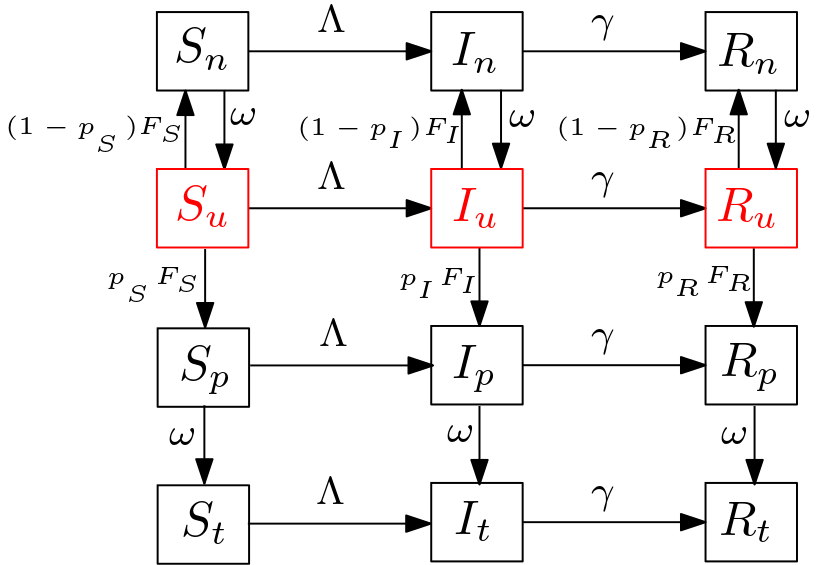
\includegraphics[scale=0.3]{./pix/sir_comp.png}
\caption{\small Flowchart of the SIR (Susceptible-Infectious-Recovered) model, \crefrange{eq1}{eq12}. For the description of the parameters see \cref{tab:params}.
\label{fig:flowchart}}
\end{center} 
\end{figure}

\jd{It would be nice to modularize the model somehow, but probably not worth anyone's time.}

\ali{not sure if these should go to the Supp material?} In our model the following parameters are used (for a summery of parameters' description, see Table \ref{tab:params}). $N_0$ is the total population size, $\omega$, (1/day), is the rate of onward flow from the awaiting positive or negative compartments to reported or untested compartments, respectively, $\gamma$, (1/day), is the recovery rate, $\rho$, (1/day), is the per capita testing intensity across the whole population. Further, various testing strategies are incorporated through the compartment-specific relative testing weights $W_S$, $W_I$ and $W_R$. What matters in these weight is their relative proportions. For example, $W_I/W_S=2$ means that, the probability that infected individuals get tested is as twice as that of susceptible individuals. The weighted number of people available for tests is defined as $W = W_S S_u + W_I I_u + W_R R_u$, and the scaling parameter for testing defined as

\begin{equation}
\label{sigma}
\sigma = \frac{\rho N_0}{W}.
\end{equation}
Thus, the weighted testing rate is defined as $F_Z=\sigma W_Z$, where $Z \in \{S,I,R\}$. Note that requiring a fixed testing rate as in \eqref{sigma} can lead to a singularity when no one is left untested. We discuss this issue, and a practical solution, in the Appendix. 

The classical SIR model is based on the following implicit assumptions (see a ref for details); well-mixed population, homogeneity of the population, exponentially distributed duration of infection and large population size (may be refer the reader to \cite{keeling2011modeling}). In addition to these standard assumptions, our model, \crefrange{eq1}{eq12}, assumes: (i) there is a single force of infection, $\Lambda$, that is, where a susceptible individual moves to does not depend on who infected it, (ii) $\eta_c \leq \eta_w$, i.e., the individuals awaiting test results have a higher transmission probability than the reported individuals, (iii) a perfectly specific test, $p_S=0$, for simplicity in analysis. Note that the latter assumption combined with the assumption that the total population was initially distributed between untested and awaiting for negative test, that is $S_u+S_n=0$, reduce the model to 10 equations with equations \ref{eq3} and \ref{eq4} are eliminated. Specifically, when the population is at steady states and the number of infected people is negligible, the assumption of perfect specificity results in $S_p=0$ in \cref{eq3} and $d S_c/dt=0$ from \cref{eq4}. Also, since we assumed $S_u+S_n=0$, initially $S_c=0$ and stays in this state.

\newgeometry{margin=1cm} % modify this if you need even more space
\begin{landscape}
\begin{table}[htp]
\centering
{\tiny %
\begin{tabular}{|c|ccc|} \hline
  Symbol & Description & Unit & Value \\ \hline
  $N_0$     & Total population size & people & $10^6$ \\ \hline
  $\omega$  & Rate of onward flow from the awaiting to reported or untested compartments  & 1/day & - \\ \hline
  $\gamma$ & Recovery rate & 1/day & 1/3 \\ \hline 
  $\rho$   & Per capita testing intensity & 1/day & 0.01 \\ \hline 
  $\eta_w$  & Relative probability of transmission for isolated awaiting individuals & - & - \\ \hline
  $\eta_c$  & Relative probability of transmission for isolated confirmed individuals & - & -  \\ \hline
  $\Lambda$ & Force of infection & 1/day & - \\ \hline
  $p_S$ & Probability of false positive for susceptible& - & 0 \\ \hline
  $p_I$ & Probability of being infected and tested positive & - & 1 \\ \hline
  $p_R$ & Probability of being recovered and tested positive & - & 0.5 \\ \hline
  $W_S, W_I, W_R$ & Relative testing weight & - & 
  \begin{minipage}[t]{0.21\columnwidth}%
 Random testing: $W_S=W_I=W_R=1$, \\Non-random testing: $W_S=0.3, W_I=W_R=1$
\end{minipage} \\ \hline

  \end{tabular}
  }%
\caption{\label{tab:params} The underlying parameters of model, \crefrange{eq1}{eq12}.}
\end{table}
\end{landscape}
\restoregeometry


The Disease-Free Equilibrium (DFE) for the SIR model, \crefrange{eq1}{eq12}, is given by solving the coupled system including $S_u+S_n=N_0$ and $F_S S_u-\omega S_n=0$. The DFE is

\begin{equation}
\label{dfe}
S_n^*= \frac{\rho}{\omega} N_0, \ S_u^*= N_0-S_n^*, \text{and} I_j=R_j=0 \ \text{for all j}.
\end{equation}

The basic reproduction number, $\Rnum$, was calculated by using the next generation matrix method developed by \cite{van2002reproduction}. $\Rnum$ is

\begin{equation}
\label{R0}
\Rnum= (A \times S_u^* + B \times S_n^*) \times C, 
\end{equation}
where
\begin{align*}
A=& \gamma(\omega+\gamma) + (\gamma \eta_w + \omega \eta_c p_I) F_I, \\
B=& \big(\omega+(F_I+\gamma)\eta_w\big) \gamma+\frac{(\eta_w \gamma+ \eta_c\omega) \omega p_I F_I }{\omega+\gamma}, \\ 
C=& \frac{\beta/\gamma}{N_0 (\gamma(\omega+\gamma)+F_I(\gamma+\omega p_I))}.
\end{align*}

Further details are provided in the Appendix.
 
\todo{Something needs to be said here about simulation part.} The analytical calculation of the next generation matrix, $G$, and the derivation of $\Rnum$ was carried out in Maple (ref) by using simple linear Algebra package. 
  We used \Rlogo for the simulation part which included using the explicit expression of $\Rnum$ \ref{R0} as a function of the underlying parameters, specifying the parameters a realistic range, calculating the corresponding $\Rnum$ and plotting the contours of $\Rnum$ by using ggplot package in \Rlogo. The related result is presented in Figure \ref{pan}, where  panel \eqref{p.a} represents the random testing, and panel \eqref{p.b} is representing non-random testing. The parameter values or ranges are as follows (I like using a table here, with the param, their units and values). It is notable that in the simulation part, the explicit expression of $\Rnum$ was used and not the approximation \eqref{eq:R0appr}. This simulation reflects the behavior of $\Rnum$ with respect to the selected parameters for two different testing strategies: (i) random testing, represented by all testing weights to be the same, $W_S=W_I=W_R$, and (ii) non-random testing, when testing weight are not equal. For simulation purposes we chose $W_S=W_I=W_R=1$ for random testing, and $W_S=0.3$ and $W_I=W_R=1$ for non-random testing strategy. Note that the critical contour of $\Rnum=1$ is plotted in solid line in Figure \ref{pan}. 


% %%%%%%%
\section{Results}

The explicit formula for the basic reproduction number, $\Rnum$ \eqref{R0}, provides an opportunity to study the influence of changes in the underlying parameters on the critical index of epidemic dynamics. We are interested in understanding the effect of parameters that can be realistically controlled by changing in isolation, testing intensity and test resulting, i.e., $\eta_c$ and $\eta_w$, $\rho$ and $\omega$, respectively. The following Proposition is the direct result of taking partial derivative of $\Rnum$ \eqref{R0} with respect to selected parameters. 

\begin{proposition}
\label{prop1}
Using the expression of $\Rnum$ \eqref{R0},
\begin{enumerate}
\item \label{p1:eta}
$\partial{R_0}/\partial{\eta_c} \geq 0$ and $\partial{R_0}/\partial{\eta_w} \geq 0$. 
\item \label{p1:rho}
$\partial{\Rnum}/\partial{\rho} \leq 0$ when $\rho \approx 0$.
\item \label{p1:omega}
$\partial{R_0}/\partial{\omega}$ can be positive or negative when $\rho \approx 0$.
\end{enumerate}
\end{proposition}

 Given that the perfect isolation occurs at $\eta_c=\eta_w = 0$, Prop. \ref{p1:eta} means that lifting the isolation from awaiting group results in an increased $\Rnum$ and consequently a greater number of infected individuals. We used Taylor approximation of $\Rnum$ at $\rho=0$ due to the complexity of the expression and thus inconclusive. See the Appendix for details. It is straightforward to derive \ref{p1:rho} and \ref{p1:omega} from the linear approximation of $\Rnum$ at $\rho=0$.
 
 Prop. \ref{p1:rho} indicates that increasing testing intensity reduces the $\Rnum$. This is sensible since as people are moved to test compartments ($I_p$, $I_n$ \fady{the susceptibles also reduce contact and transmission}) the higher probability of being subject to isolation and the lower the transmission \eqref{Lambda} will become.
 
 Of these results, prop. \ref{p1:omega} is the most surprising. It states that returning test results more rapidly (i.e., increasing $\omega$) does not necessarily lower $\Rnum$, rather, whether increasing $\omega$ lowers $\Rnum$ is defendant on the precise combination of model parameters (test reporting rate itself, testing processes/strategies ($W$'s), testing efficacy ($P_I$) and isolation ($\eta$'s). Specifically, the $\partial{R_0}/\partial{\omega}>0$ suggests that reproduction number may increase as the test reporting process become faster. This can be seen from expression \eqref{Rom} in the case of ``perfect isolation``, when $\eta_w=0$ and $\eta_c=0$. The underlying mechanism for this result is that individuals may take more precautionary behaviors (e.g., physical distancing) when they are awaiting test results compared to when they are untested or their test has returned negative. An example of a situation that would favour slow return of tests is if the test being employed produces many false negatives, because many infected individuals will believe they are negative and thus may unknowingly spread the virus to many others.  For an example of the behaviour of $\Rnum$ see Figure \ref{pan} at varying values of $\omega$. This property also provides a tool to quantify the amount of delay required in the test reporting process as a strategy to reduce $\Rnum$ and consequently control the epidemic.   

[comments about the figure:]
1- use a single legend, change the range manually.
\begin{figure}[h!]
\centering
\begin{subfigure}[t]{.45\textwidth}
\centering
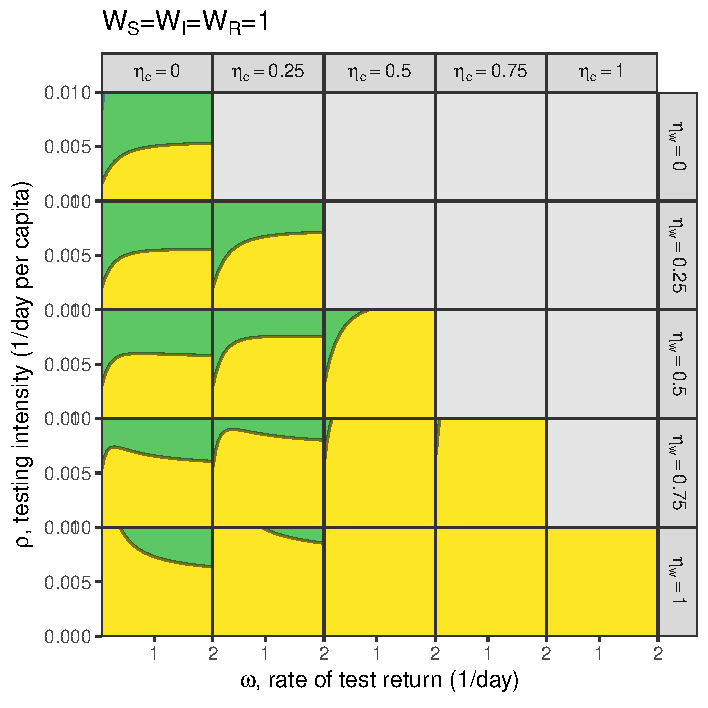
\includegraphics[width=\linewidth]{./pix/R0contour_random.pdf}
\caption{}\label{p.a}
\end{subfigure}
%
\begin{subfigure}[t]{.45\textwidth}
\centering
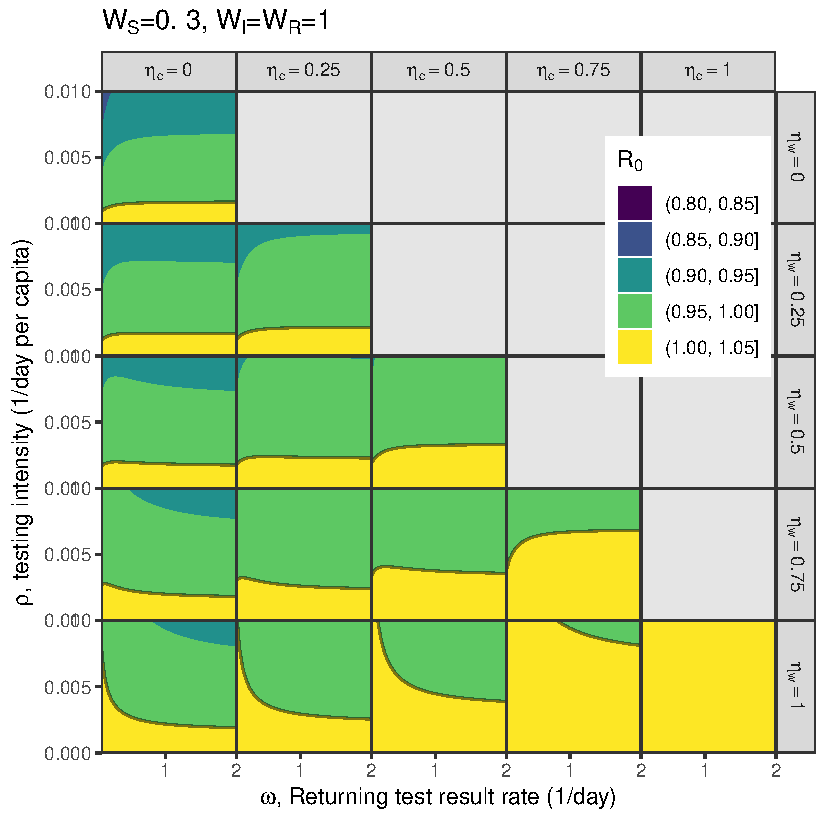
\includegraphics[width=\linewidth]{./pix/R0contour_TTI.pdf}
\caption{}\label{p.b}
\end{subfigure}
\caption{Behaviour of the basic reproduction number, $\Rnum$, with respect to changes in the underlying parameters; remind the reader about the parameters and their values in this simulations. the solid line in each panel represents the critical contour of $\Rnum=1$.}
\label{pan}
\end{figure}

Our numerical simulation in support of the analytical results in Proposition \ref{prop1} are presented in Figure \ref{pan}. It can be inferred that when random testing strategy is applied, Figure \ref{p.a}, comparing to the non-random testing strategy, Figure \ref{p.a}, the critical testing intensity of the corresponding panels are lower in non-random testing. Also, it appears that speeding the test reporting, i.e., increasing $\omega$, does not significantly lower $\Rnum$ when awaiting people follow the isolation perfectly, i.e., $\eta_w$ is closer to 0. However, speeding the test reporting reduces the epidemic more when the awaiting people less follow the isolation, i.e., $\eta_w$ is closer to 1. 

Furthermore, we derived an inequality that quantifies the exact relationships between model parameters that result in returning tests more rapidly being favorable \eqref{eq:necsuf}. To give a biological interpretation, we describe the qualitative \textit{trends} predicted by the inequality. Returning test results more rapidly \textit{tends} to be more favorable when

\begin{itemize}
    \item individuals who have tested positive lower their contact much more than individuals who are waiting for their test results (i.e., $\eta_c \ll \eta_w$).
    \item the test is sensitive.
    \item testing of infected individuals is more intense than testing of susceptible individuals.
\end{itemize}
An in-depth discussion of these results is presented in the discussion section. 

The use of tests cheaper than RT-PCR has been proposed as a potential strategy for containing the COVID-19 pandemic. While cheaper tests may be less sensitive and reliable than RT-PCR, they allow for broader and more intense testing. Using our Taylor approximation of $\Rnum$ near $\rho = 0$, we examined what circumstances (i.e., model parameters) make the use of one test more favourable than another, and give a complete description through inequality \ref{eq:rho1vsrho2}. In general, we found that the expensive test \textit{tends} to more effectively lower $\Rnum$ when

\begin{itemize}
    \item individuals who test positive self-isolate much more than individuals who are waiting for their test result.
    \item the time it takes to return tests is much shorter than the mean infectious period.
    \item the testing intensity is much greater for infected individuals than susceptible individuals.
\end{itemize}

Our model also predicts an asymmetry between cheap and expensive tests: if a cheap test can identify on average more infected individuals as an expensive test, then our model predicts that the cheap test will lower $\Rnum$ more. In contrast, if an expensive test can identify on average more infected individuals, it will not necessarily lower $\Rnum$ more than the cheap test. \fady{we can state this as a formal proposition in equations rather than in words, if that would be better.}

%%%%%%%%%%%%

% %%%%%%%
\section{Discussion}

- JD's email:
We're basically looking at the potential advantage of slow tests:
people waiting for test results may be more careful than those who
have received negatives. These advantages are real, and neglected. We
also compare to an individual-level advantage of fast tests: people
who test positive may be even more careful. But we are missing out on
community-level advantages of fast testing: better assessment of the
situation, identification of hot spots, contact-tracing, etc. 

- May be something about the testing rate/intensity, now the per capita testing intensity is very low ($\rho \approx 0$). In near future new test kits may be widely accessible, our model provide insights in this case (what are those?)

- "delay negative results" result

\subsection{Rate of returning tests}

Our model predicts that when the difference in self-isolation between individuals waiting for their tests and individuals who are confirmed positive is small, returning tests rapidly is not beneficial. The underlying mechanism for this prediction is that the benefit in returning tests rapidly so (i.e., the extra self-isolation an individual does when they test positive) is minimal and outweighed by the fact that those who test negative may increase their contacts. Thus, in such a case, returning tests more rapidly is expected to increase $\Rnum$. Similarly, if the test is not sensitive, many infected individuals will test negative, and thus may increase their contacts under the false belief that they are not infectious, so returning tests rapidly in this case may also contribute to increased transmission.

When testing of infected individuals is more intense than susceptible individuals, returning test results rapidly is beneficial because those infected individuals will be informed and self-isolate. Conversely, if testing of susceptible individuals is much greater, very few tests will be positive, and the benefit of informing those few positive cases will be outweighed by the potential increase in contacts of the individuals testing negative. 


\subsection{Expensive vs. cheap tests}
\fady{I think we should discuss this before I write it. I'm a little hesitant to really expand on these results because of the points JD brought up over email.}


% %%%%%%%
\bibliography{SIRlibrary.bib}

% %%%%%%%
\section{Supplementary Material}

\subsection{Model and Calculation of $\Rnum$}

The model is 
\begin{align}
% \label{model}
 d S_u/dt &= -\Lambda S_u - F_S S_u + \omega S_n, \label{eq1}\\
 d S_n/dt &= -\Lambda S_n + (1-p_S) F_S S_u - \omega S_n, \label{eq2}\\
 d S_p/dt &= -\Lambda S_p + p_S F_S S_u - \omega S_p, \label{eq3}\\
 d S_c/dt &= -\Lambda S_c + \omega S_p, \label{eq4}\\
 d I_u/dt &= \Lambda S_u - F_I I_u + \omega I_n  - \gamma I_u,  \label{eq5}\\
 d I_n/dt &= \Lambda S_n + (1-p_I) F_I I_u - \omega I_n -\gamma I_n, \label{eq6}\\
 d I_p/dt &= \Lambda S_p + p_I F_I I_u - \omega I_p -\gamma I_p, \label{eq7}\\
 d I_c/dt &= \Lambda S_c + \omega I_p - \gamma I_c,  \label{eq8}\\
 d R_u/dt &= \gamma I_u - F_R R_u + \omega R_n, \label{eq9}\\
 d R_n/dt &= \gamma I_n + (1-p_R) F_R R_u - \omega R_n,  \label{eq10}\\
 d R_p/dt &= \gamma I_p + p_R F_R R_u  - \omega R_p,  \label{eq11}\\
 d R_c/dt&= \gamma I_c + \omega R_p,  \label{eq12}\\
 dN/dt &= \omega (S_n + I_n + R_n),   \label{eq13}\\
 dP/dt &= \omega(I_p + R_p) \label{eq14},
\end{align}

where $\beta$, (in units of 1/day), is the disease transmission rate, $\eta_w$ and $\eta_c$ are the isolation parameters for awaiting and reported individuals, respectively. $\Lambda$ is the force of infection and is defined as 

\begin{equation}
\label{Lambda}
\Lambda=\beta \frac{(I_u+\eta_w I_n+\eta_w I_p+ \eta_c I_c)}{N_0},
\end{equation}

% %

The next generation matrix is $G = F V^{-1}$, where matrix $F$ represents the inflow of new infection to the infected compartments and matrix $V$ represents the flow in the infected compartments when the population is totally susceptible. For model, \crefrange{eq1}{eq12}, $F$ and $V$ are

\begin{align}
\label{FV}
F =& \beta/N_0 \left[ \begin {array}{cccc} 
S_u&\eta_w\,S_u&\eta_w\,S_u&\eta_c\,S_u\\
S_n&\eta_w\,S_n&\eta_w\,S_n&\eta_c\,S_n\\ 
0&0&0&0\\
0&0&0&0
 \end {array} \right], \\
  V =&
 \left[ \begin {array}{cccc}  
F_I+\gamma&-\omega&0&0\\
-(1-p_I)F_I&\omega+\gamma&0&0\\
-p_I F_I&0&\omega+\gamma&0\\
0&0&-\omega&\gamma
\end {array} \right], \text{thus}\\
V^{-1} =&
\left[ \begin {array}{cccc}
\frac {\omega+\gamma}{\omega\,\gamma+\gamma F_I+\gamma^2+\omega\, F_I p_I}&\frac {\omega}{\omega\,\gamma+\gamma F_I+\gamma^2+\omega\, F_I p_I}&0&0\\
\noalign{\medskip}
\frac{(1-p_I) F_I}{\omega\,\gamma+\gamma F_I+\gamma^2+\omega\, F_I p_I}&
\frac{F_I+\gamma}{\omega\,\gamma+\gamma F_I+\gamma^2+\omega\, F_I p_I}&0&0\\
\noalign{\medskip}
\frac{p_I F_I}{\omega\,\gamma+\gamma F_I+\gamma^2+\omega\, F_I p_I}&
\frac{\omega p_I F_I}{(\omega\,\gamma+\gamma F_I+\gamma^2+\omega\, F_I p_I)(\omega+\gamma)}& \frac{1}{\omega+\gamma}&0 \\
\noalign{\medskip}
\frac{\omega\,F_I\,p_I}{(\omega\,\gamma+\gamma F_I+\gamma^2+\omega\, F_I p_I) \gamma}& 
\frac{\omega^2\,F_I\,p_I}{(\omega\,\gamma+\gamma F_I+\gamma^2+\omega\, F_I p_I)(\omega+\gamma) \gamma}&
\frac{\omega}{(\omega+\gamma) \gamma}&
\frac{1}{\gamma}
\end {array} \right].
\end{align}

The particular form of $F$ with two rows of zeros at the bottom, simplifies $G$ as 
\begin{equation}
G = \left[ \begin {array}{cc}
G_{11}&G_{12}\\
0&0
\end {array} \right], \text{ where } \\
G_{11} =C
\left[\begin {array}{cc}
A\,S_u & B\,S_u\\
A\,S_n & B\,S_n
\end {array}\right].
\end{equation}

Note that the block matrix $G_{12}$ does not influence $\Rnum$ defined as the spectral radius of $G$. All matters here are the eigenvalues of $G_{11}$, which are 0 and $\Rnum$ \eqref{R0}.

% %%%%%%%
\subsection{On Testing Rate and Numerical Singularity}
The testing rate, $\sigma$, should be formulated such that people from the untested compartments will not be tested if they are not there. The numerical singularity issue with the chosen $\sigma$ \eqref{sigma} is that the population in $S$ compartments appeared to blow up when the DFE is achieved. This is once the only untested people are susceptibles, the FOI will become $\Lambda=0$, testing rate $F_s=\rho N_0/S_u$. Thus, eq(1) of the model will be $d S_u/dt = - \rho N_0 + \omega S_n$ which is no longer dependent on $S_u$ and a linear rate of leaving the $S_u$ compartment.

One way to fix this issue, is to consider a maximum testing rate, $\tau$ (1/day). In general, we want to test at a rate of $\rho$ across the whole population. This won't always be possible, so we impose a maximum rate of $\tau$ per testable person and redefine $\sigma = \frac{\tau \rho N_0}{\tau W + \rho N_0}$, with the assumption that $\tau \gg \rho$. This alteration in $\sigma$, does not change any results related to $\Rnum$, thus we only impose it in the simulation of the epidemic dynamic.

% %%%%%%%
\subsection{Taylor Approximation of $\Rnum$ at $\rho=0$ }

The basic reproduction number, $\Rnum$, close to $\rho=0$ can be approximated linearly in $\rho$ by using Taylor approximation. it follows

\begin{equation}
\label{eq:R0appr}
R_0 \approx \beta/\gamma + \frac{\beta \rho}{\omega (\omega+\gamma) \gamma^2 W_S} \Big(\gamma(\eta_w-1)(\gamma W_S+\omega W_I) + (\eta_c -1)P_iW_i \omega^2 \Big) + \mathcal{O}(\rho^2).
\end{equation}

Also, to analyze the influence of $\omega$ on $\Rnum$, the approximation \eqref{eq:R0appr} was used. Then it is straight forward to have

\begin{equation}
\label{Rom}
\partial{R_0}/\partial{\omega}=  \frac{-\beta \rho}{\gamma W_S\omega^2 (\gamma+\omega)^2}  (a \omega^2 + b \omega + c),
\end{equation}

where $a=(\eta_w-1)W_I-(\eta_c-1)P_I W_I = ((s-p_I)\eta_c + (p_I-1)) W_I$, $b=2(\eta_w-1)\gamma W_S$ and $c=(\eta_w-1)\gamma^2 W_S$.
Given that $0 \leq \eta_c\leq \eta_w \leq 1 $, one can easily derive $b\leq 0$ and $c \leq 0$. 

Note that in general, the necessary and sufficient condition for $a \geq 0$ is $(s-p_I) \eta_c \geq (1-p_I)$, where $s=\frac{\eta_w}{\eta_c} \geq 1$. 

Note that in case of ``perfect isolation``, i.e., when $\eta_w=0$ and consequently $\eta_c=0$, it is straight forward to see that $a \leq 0$, $b<0$ and $c<0$. Thus, $\partial{\Rnum}/\partial{\omega} \geq 0$. 
As an example, in the case of a very accurate testing regime,  i.e., $P_I=1$, $a \geq 0$ is achieved. If $a\geq 0$, the quadratic expression in \eqref{Rom}, has Real roots. Assuming that $\omega_1<0$ and $\omega_2>0$ be the roots of the quadratic expression in $\partial{R_0}/\partial{\omega}$. Thus, $\partial{R_0}/\partial{\omega}>0$ for $0<\omega<\omega_2$ and  $\partial{R_0}/\partial{\omega}<0$ for $\omega>\omega_2$.

% %%%%%%%
[Fady: this subsection and most of the next belong to the Appendix since they are very detailed. Would you clean up the writing, there are some repeated expressions that can be referenced?]

\subsection{rate of returning tests}
The linearization of $\Rnum$ around $\rho=0$ is
\begin{equation}\label{linearization}
\Rnum \approx \beta/\gamma + \frac{\beta \rho}{\omega (\omega+\gamma) \gamma^2 W_s} \Big(\gamma(\eta_w-1)(\gamma W_s+\omega W_i) + (\eta_c -1)P_iW_i \omega^2 \Big). 
\end{equation}

So when $\rho \approx 0$ we have $$\partial{\Rnum}/\partial{\omega} \approx  \frac{-\beta \rho}{\gamma W_s\omega^2 (\gamma+\omega)^2}  (a \omega^2 + b \omega + c).$$

where $a=(\eta_w-1)W_i-(\eta_c-1)P_iW_i$, $b=2(\eta_w-1)\gamma W_s$ and $c=(\eta_w-1)\gamma^2 W_s$. 

Perhaps counter-intuitively, the equation above does not predict that $\Rnum$ is monotone decreasing with respect to $\omega$. In other words; our model does not predict that returning test results more rapidly \textit{always} lower $\Rnum$. In order to gain insight into this intriguing behavior, we examine the zeroes of $\frac{\partial{\Rnum}}{\partial{\omega}}(\omega)$.

Defining the following quantity, $Q$, will help us write the roots of $\partial{\Rnum}/\partial{\omega}$ neatly. 
\begin{align}\label{eq:defQ}
    Q =& \frac{W_i}{W_s}\left(1-\frac{n_{t}-1}{n_{w}-1}P_{i}\right) \\
\end{align}

With that in mind, we can write the roots of $\partial{\Rnum}/\partial{\omega}$ as

\begin{align}
    \omega_1 =& \frac{\gamma}{-\sqrt{1-Q}-1} \\
    \omega_2 =& \frac{\gamma}{\sqrt{1-Q}-1}
\end{align}

Note that the zeroes are real if and only if $Q < 1$. Note that have $\eta_c < \eta_w$, so if $P_i \approx 1$, we will have $Q < 0 < 1$. Thus, if we assume near-perfect test sensitivity, $\omega_1$ and $\omega_2$ will be real. 

Assuming $\omega_1, \omega_2$ are real, it is easy to confirm that $\omega_1 < 0$ by looking at the denominator. To see that $\omega_2 > 0$, recall that $Q < 0$, so $\sqrt{1-Q} > 1$ and so $\sqrt{1-Q} -1 > 0$. Knowing that $\omega_1 < 0$, the only root of interest (i.e., biologically relevant quantity) is $\omega_2$. 

We can prove that $\partial{\Rnum}/\partial{\omega} > 0$ when $\omega \in (0,\omega_2)$ and $\partial{\Rnum}/\partial{\omega} < 0$ when $\omega \in (\omega_2,\infty)$ by computing the limits of $\partial{\Rnum}/\partial{\omega}$ at $0$ and $\infty$ respectively. So it follows that $\Rnum$ has a global maximum with respect to $\omega$ at $\omega = \omega_2$.

Now we want to characterize the parameter regions on which $\partial{\Rnum}/\partial{\omega} < 0$ (i.e., the conditions under which returning test results more rapidly is favorable). By the previous analysis, this is equivalent to solving for $\omega > \omega_2$. So

\begin{align}\label{eq:necsuf}
    &\omega > \omega_2 \nonumber \\
    &\omega > \frac{\gamma}{\sqrt{1-Q}-1} \nonumber \\
    &\vdots \nonumber \\
    &\frac{1-n_{t}}{1-n_{w}}P_{i}>\frac{W_{s}}{W_{i}}\left(\frac{\gamma}{\omega}+1\right)^{2}
\end{align}


\subsection{Expensive vs. cheap tests}

The use of tests cheaper than RT-PCR has been proposed as a potential strategy for containing the COVID-19 pandemic. While cheaper tests may be less sensitive and reliable than RT-PCR, they allow for broader and more intense testing. In the analysis below, we compare the $\Rnum$ predicted by our model depending on the testing strategy. 

Consider a test that allows us to test at rate $\rho_1$ and has sensitivity $P_{i,1}$, and another test that allows us to test at $\rho_2$ and has sensitivity $P_{i,2}$. Suppose that $\rho_1 > \rho_2$. Recall that the linearization of $\Rnum$ around $\rho \approx 0$ is given by $$\Rnum \approx \beta/\gamma + \frac{\beta \rho}{\omega (\omega+\gamma) \gamma^2 W_s} \Big(\gamma(\eta_w-1)(\gamma W_s+\omega W_i) + (\eta_c -1)P_iW_i \omega^2 \Big).$$


Treating $\Rnum$ as a function of $\rho$ and $P_i$,we can reduce the inequality $$\Rnum(\rho_2, P_{i,2}) < \Rnum(\rho_1, P_{i,1})$$ into 

\begin{align}\label{eq:rho1vsrho2}
    &\rho_1\left(\gamma(\eta_w-1)(\gamma W_s + \omega W_i) + (\eta_c-1)P_{i, 1}W_i\omega^2\right) - \rho_2\left(\gamma(\eta_w-1)(\gamma W_s + \omega W_i) + (\eta_c-1)P_{i, 2}W_i\omega^2\right) > 0 \nonumber \\
    &\vdots \nonumber \\
    &\frac{\rho_2P_{i, 2}-\rho_1P_{i, 1} }{\rho_1-\rho_2} > \frac{1-\eta_w}{1-\eta_c}\cdot \frac{\gamma(\gamma W_s + \omega W_i)}{\omega^2 W_i}
\end{align}

Note that the RHS is positive, thus a necessary condition for the inequality above to hold is that $\rho_2P_{i,2} > \rho_1P_{i,1}$, equivalently 

\begin{equation}
\frac{P_{i,2}}{P_{i,1}} > \frac{\rho_1}{\rho_2}.
\end{equation}

To state an example of this, if test $A$ is three times as expensive as test $B$ (and hence one can test three times as many people with test $B$), using test $A$ rather than $B$ will be favorable only if test $A$ is at least 3 times more sensitive than test $B$. Note that this is a necessary but not sufficient condition, so even if test $A$ is three times more sensitive, it is still possible for test $B$ to be more effective. 

\cref{eq:rho1vsrho2} tells us precisely when a test corresponding to $\rho_2, P_{i,2}$ will yield a lower $\Rnum$ than a test corresponding to $\rho_1, P_{i,1}$, where $\rho_1 > \rho_2$. Some of the qualitative \textit{trends} that favor test 2 (the higher-sensitivity test) include

\begin{itemize}
    \item individuals who test positive self-isolate much more than individuals who are waiting for their test result.
    \item the time it takes to return tests is much shorter than the mean infectious period.
    \item the testing intensity is much greater for infected individuals than susceptible individuals.
\end{itemize}


% %%%%%%%
\subsection{Literature Review}

\subsubsection{Explicit models of TTI (trace/test/isolate) based on network or agent-based models}
\citep{endo2020implication} \ali{It seems to me that this is just a statistical model to estimate the parent-offspring of an infected index, not sure if it fits into agent-based group!} Used simulation on a branching process model to assess the forward and backward contact tracing efficiency. Assuming a negative-binomial branching process with a mean R, reproduction number, and overdispersion parameter k, the mean total number of generation G3 and averted G3 are estimated. The effectiveness of TTI is defined as the ratio of averted to the mean.

\citep{jenness2020modeling} developed a network-based transmission model for SARS-CoV-2 on the Diamond Princess outbreak to characterize transmission dynamics and to estimate the epidemiological impact of outbreak control and prevention measures. 

\citep{elbanna2020entry} [seems similar to MacPan model!]

\citep{de2020influenza} Was discussed in the Math 747 
SEIR Asymptomatic and symptomatic $I_1, I_2$. Used linear chain trick 
Stringency index as a control force lowering $\beta$.

\citep{rice2020effect} Effect of school closures on mortality. Reproduce Report 9 results by spatial agent based CovidSim. 
% %%%%%%%
\subsubsection{Models of repeated random testing of isolated populations}
\cite{bergstrom2020frequency}
(1) Model, assumptions: They developed a function, namely expected exposure $E(C,\tau)$, to approximate trade-offs between the frequency of testing, n, the sensitivity of testing, q, and the delay between
testing and results, d. This function is explicitly derived and was connected the effective reproduction number $R=R_0 S$, where $S$ is the proportion of population susceptible.
assumption that transmission rates are a step function: individuals who
have COVID go from non-infectious to fully infectious instantaneously,
and remain fully infectious until they are no longer able to transmit disease. Test sensitivity takes the same form over the course of infection.
More sophisticated models could allow varying infectiousness and varying
sensitivity over time, as in 
\citep{larremore2020test}.

\citep{lopman2020model} Used a Deterministic SEIR model, incorporated TTI, applicable to a university setting. They assumed a fairly high reproductive number that is not reduced through social
distancing measures. They found that community-introduction of SARS-CoV-2 infection onto campus can be
relatively controlled with effective testing, isolation, contract tracing and quarantine.

\citep{tuite2020mathematical} used an age-structured compartmental model of COVID-19 transmission in the population of Ontario, Canada. We compared a base case with limited testing, isolation and quarantine to different scenarios. 
% %%%%%%%
\subsubsection{Other maybe-related works}
\citep{arino2020simple} developed a SLIAR compartmental model to study the spread of an epidemic, specifically COVID-19, in a population. The model incorporates an Erlang distribution of times of sojourn in incubating, symptomatically and asymptomatically infectious compartments. Basic reproduction number is derived. Also, sensitivity analysis with respect to the underlying parameters for the following two outputs was carried out; (i) the number of observable cases during the course of the epidemic and at the peak, and (ii) the timing of the peak of the outbreak. Sensitivity analysis is performed using the R package multisensi.

\citep{ruszkiewicz2020diagnosis} novel with-in-a-minute breath testing with 80\% accuracy. 

\end{document}
